\section{共形映射-刷题}

见复变函数论 (第五版) 学习指导书 (钟玉泉编) (Z-Library)

\subsection{解析变换的保域性}

\begin{theorem}
不恒为常数的解析变换 $w=f(z)$ 是保域的,即将区域 $D$ ($f(z)$ 在 $D$ 内解析)变成区域 $f(D)$。
\end{theorem}
\begin{corollary}
单叶解析变换是保域的。
\end{corollary}
\begin{theorem}[(定理7.1的推广)]
设 $w=f(z)$ 在扩充 $z$ 平面的区域 $D$ 内除可能有极点外处处解析,且不恒为常数,则 $D$ 的像 $G=f(D)$ 为扩充 $w$ 平面上的区域。
\end{theorem}
\subsection{解析变换的保角性}

\subsubsection{导数的几何意义}

设 $f:D\to f(D)$ 解析,$z_0\in D$, $f'(z_0)\neq0$,于是 $\arg f'(z_0)$ 只与 $z_0$ 有关,与过 $z_0$ 的曲线 $C$ 无关,称为变换 $w=f(z)$ 在 $z_0$ 的旋转角. 类似的,$\lvert f'(z_0) \rvert$ 称为变换 $w=f(z)$ 在 $z_0$ 的伸缩率.

\begin{theorem}[定理 7.4]
如 $w=f(z)$ 在区域 $D$ 内解析,$z_0 \in D, f^{\prime}\left(z_0\right) \neq 0$ ,则变换 $w=$ $f(z)$ 在点 $z_0$ 处是保角的(即过 $z_0$ 的一对曲线的交角与过像点 $w_0$ 的一对像曲线的交角大小相等,方向一致);在 $D$ 内单叶解析的变换是保角的.
\end{theorem}
\subsection{圆在分式线性映射下的像}

\begin{figure}[H]
\centering
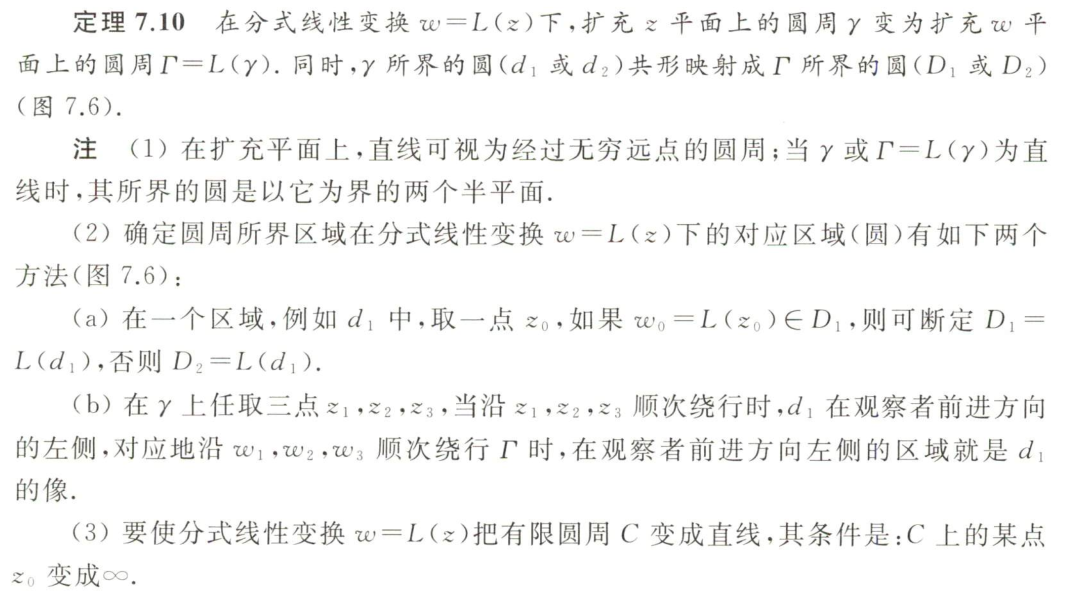
\includegraphics[width=\textwidth]{共形映射-刷题-2025060920.png}
% \caption{}
\label{}
\end{figure}
\begin{figure}[H]
\centering
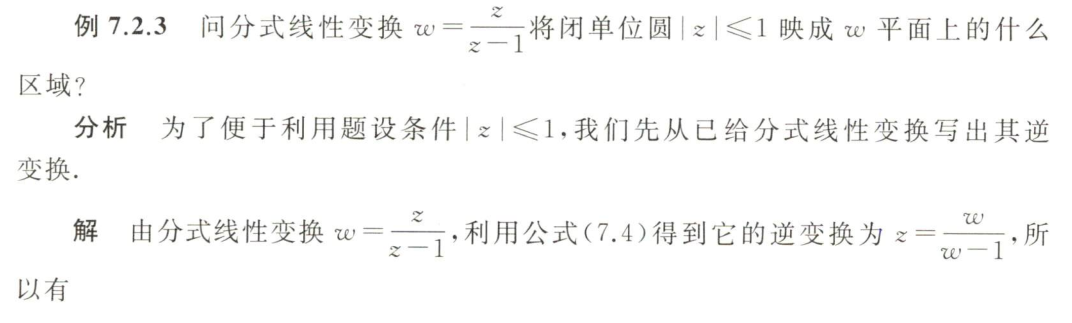
\includegraphics[width=\textwidth]{1-共形映射-刷题-2025060920.png}
% \caption{}
\label{}
\end{figure}
\begin{figure}[H]
\centering
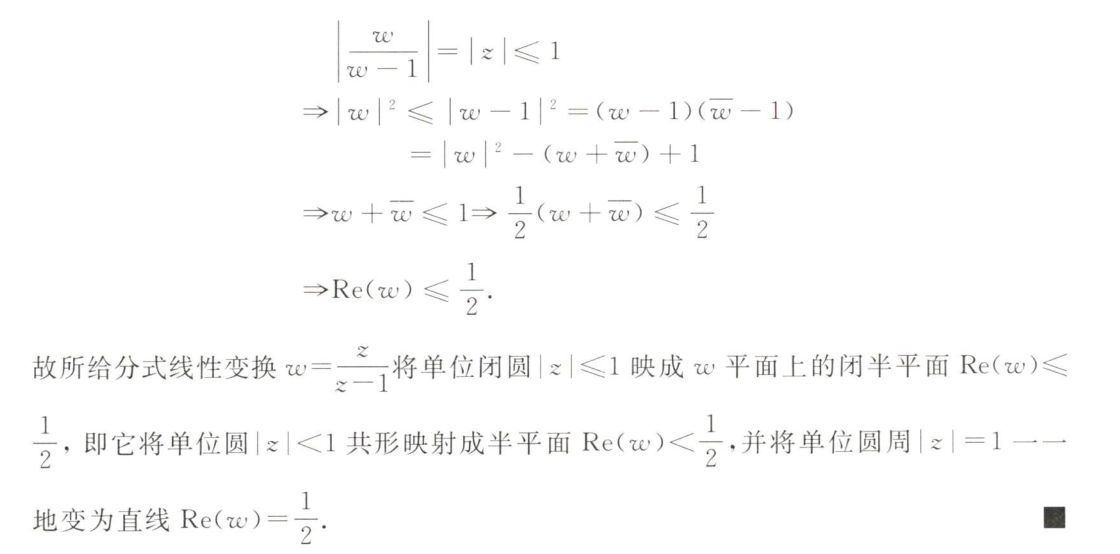
\includegraphics[width=\textwidth]{2-共形映射-刷题-2025060920.png}
% \caption{}
\label{}
\end{figure}

\subsection{圆周到圆周的分式线性映射}

\begin{figure}[H]
\centering
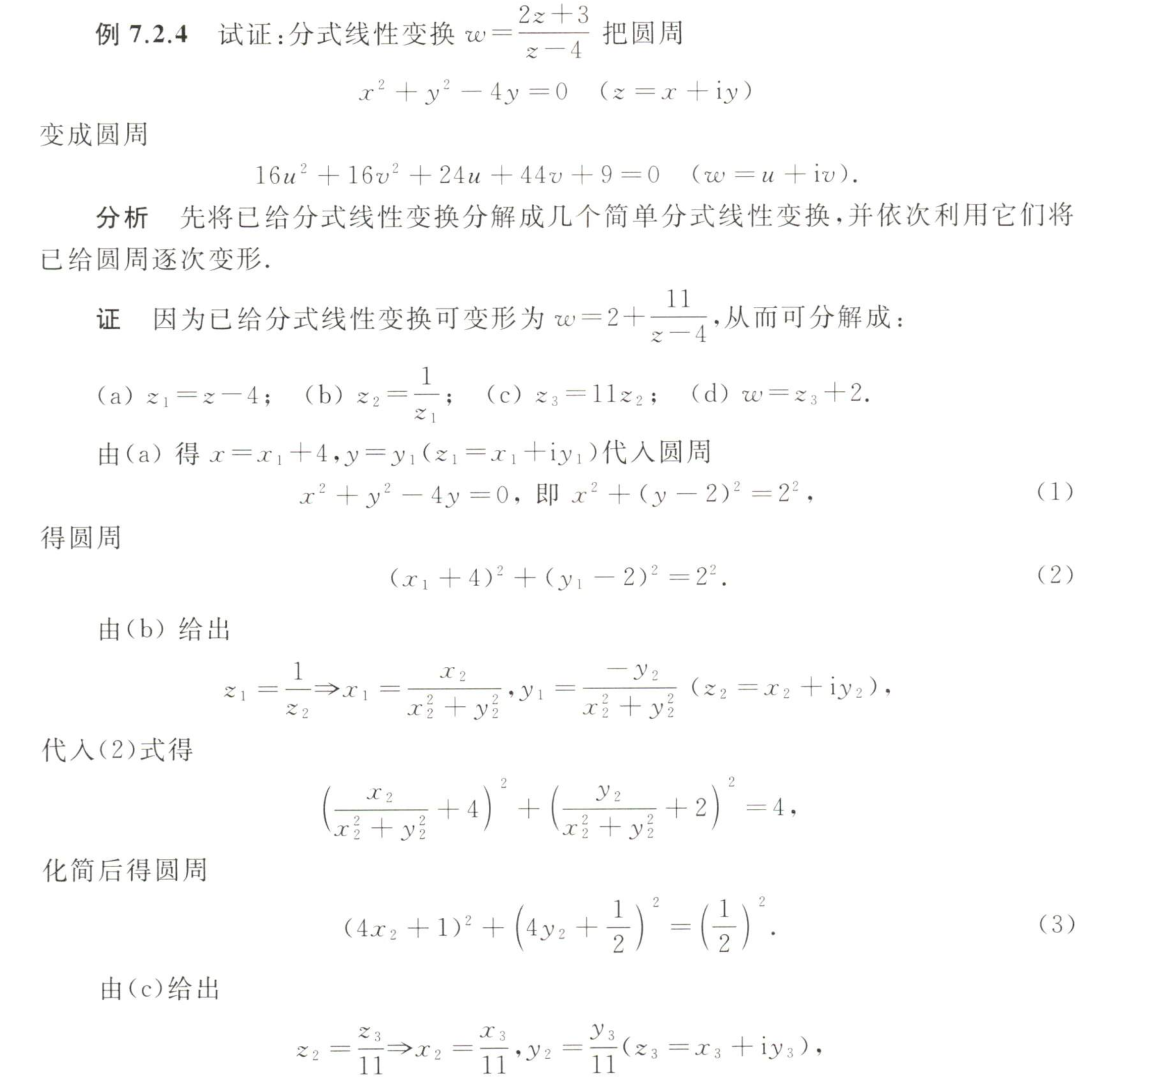
\includegraphics[width=\textwidth]{3-共形映射-刷题-2025060920.png}
% \caption{}
\label{}
\end{figure}
\begin{figure}[H]
\centering
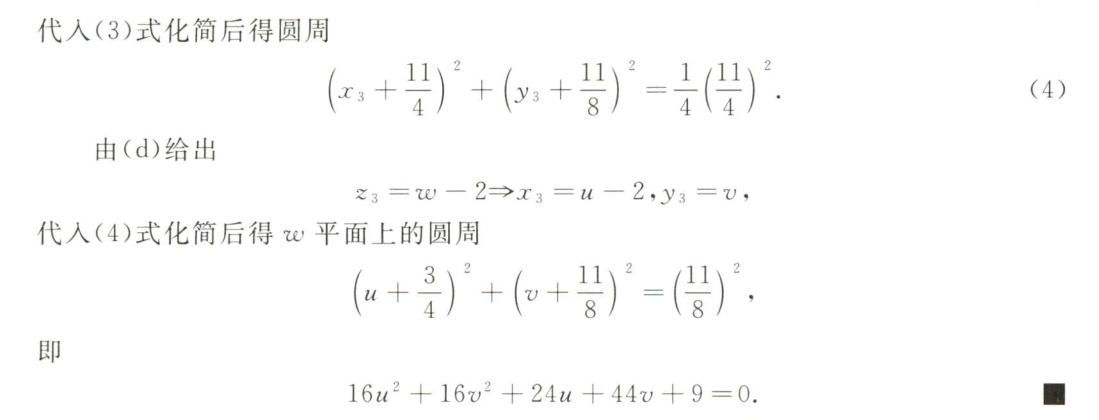
\includegraphics[width=\textwidth]{4-共形映射-刷题-2025060920.png}
% \caption{}
\label{}
\end{figure}

\subsection{给定三个对应点的分式线性映射}

使用交比,或者联立求解

交比:
\[
(z_1,z_2,z_3,z_4)=\frac{z_4-z_1}{z_4-z_2}\cdot\frac{z_3-z_2}{z_3-z_1}
\]
\begin{figure}[H]
\centering
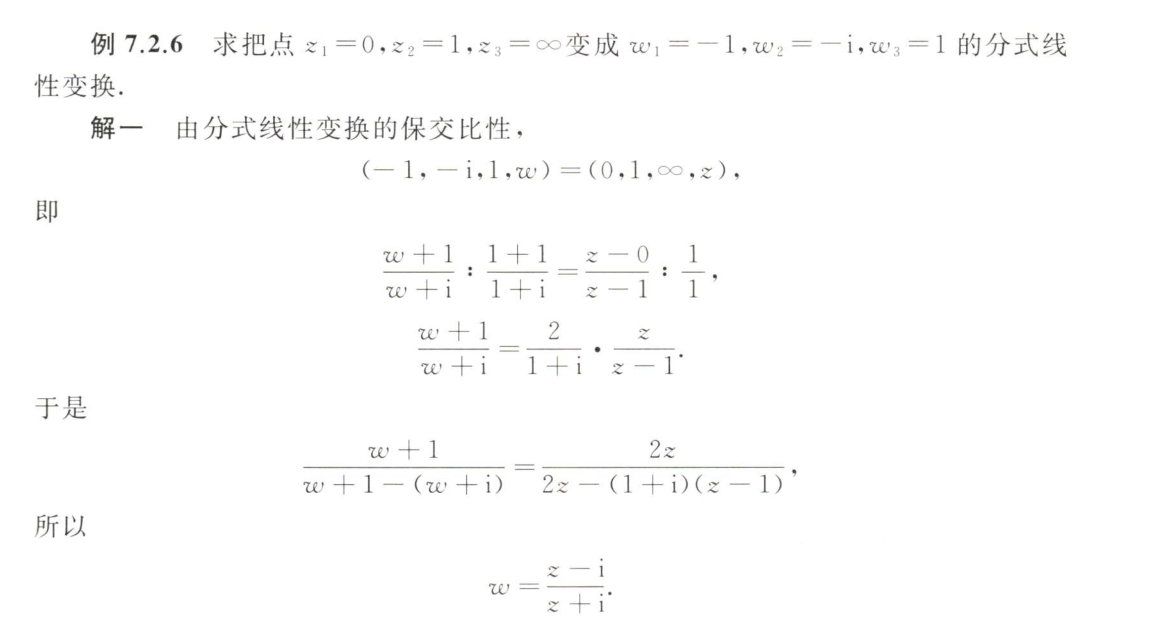
\includegraphics[width=\textwidth]{5-共形映射-刷题-2025060920.png}
% \caption{}
\label{}
\end{figure}
\begin{figure}[H]
\centering
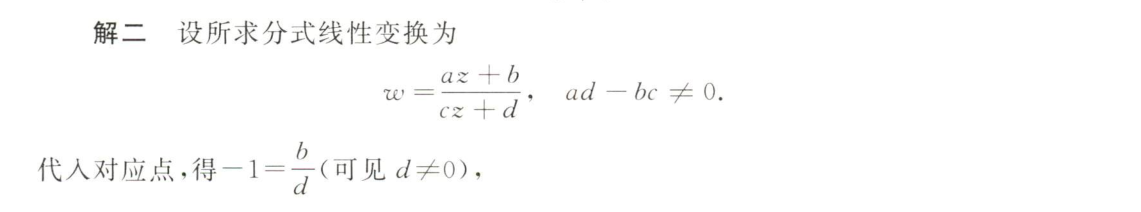
\includegraphics[width=\textwidth]{6-共形映射-刷题-2025060920.png}
% \caption{}
\label{}
\end{figure}
\begin{figure}[H]
\centering
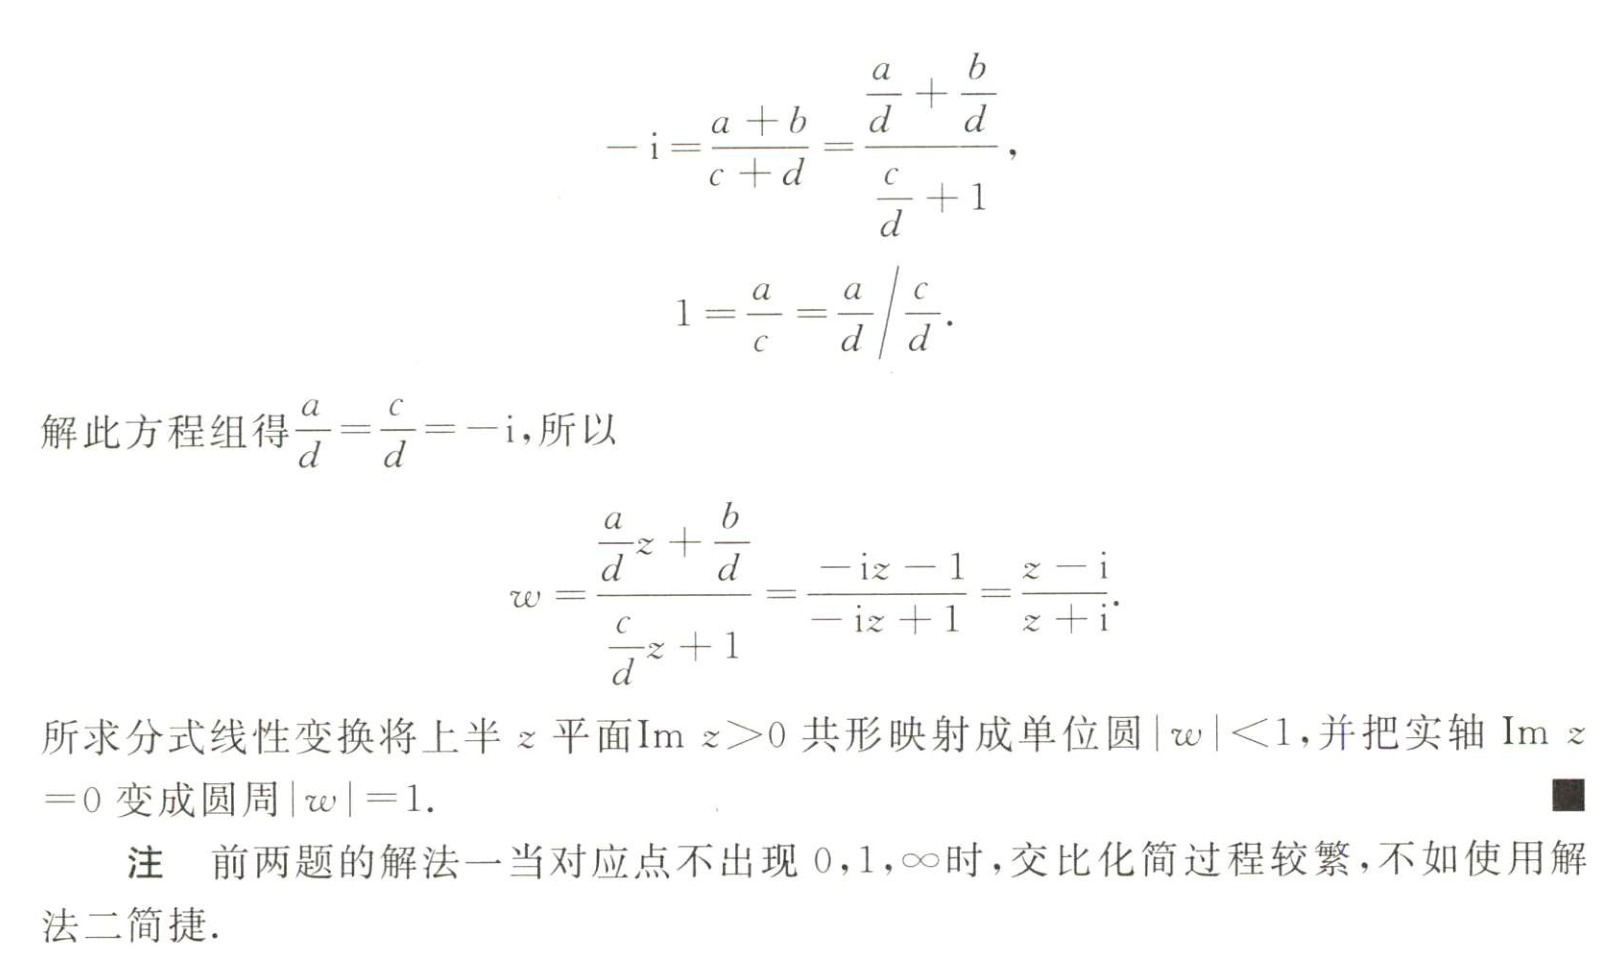
\includegraphics[width=\textwidth]{共形映射-刷题-2025060921.png}
% \caption{}
\label{}
\end{figure}

\subsection{分式线性映射保持对称点}

\begin{figure}[H]
\centering
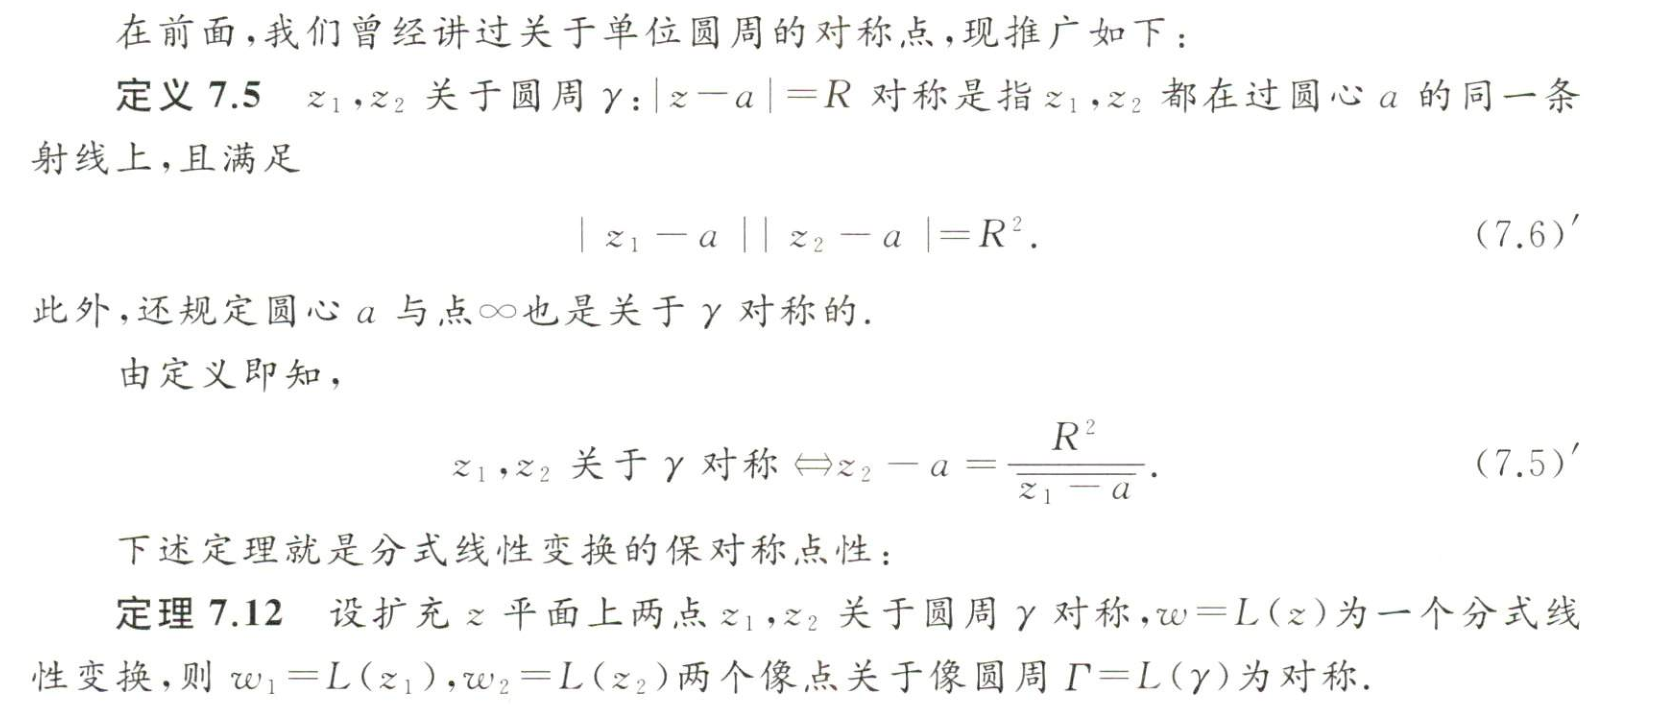
\includegraphics[width=\textwidth]{1-共形映射-刷题-2025060921.png}
% \caption{}
\label{}
\end{figure}
\begin{figure}[H]
\centering
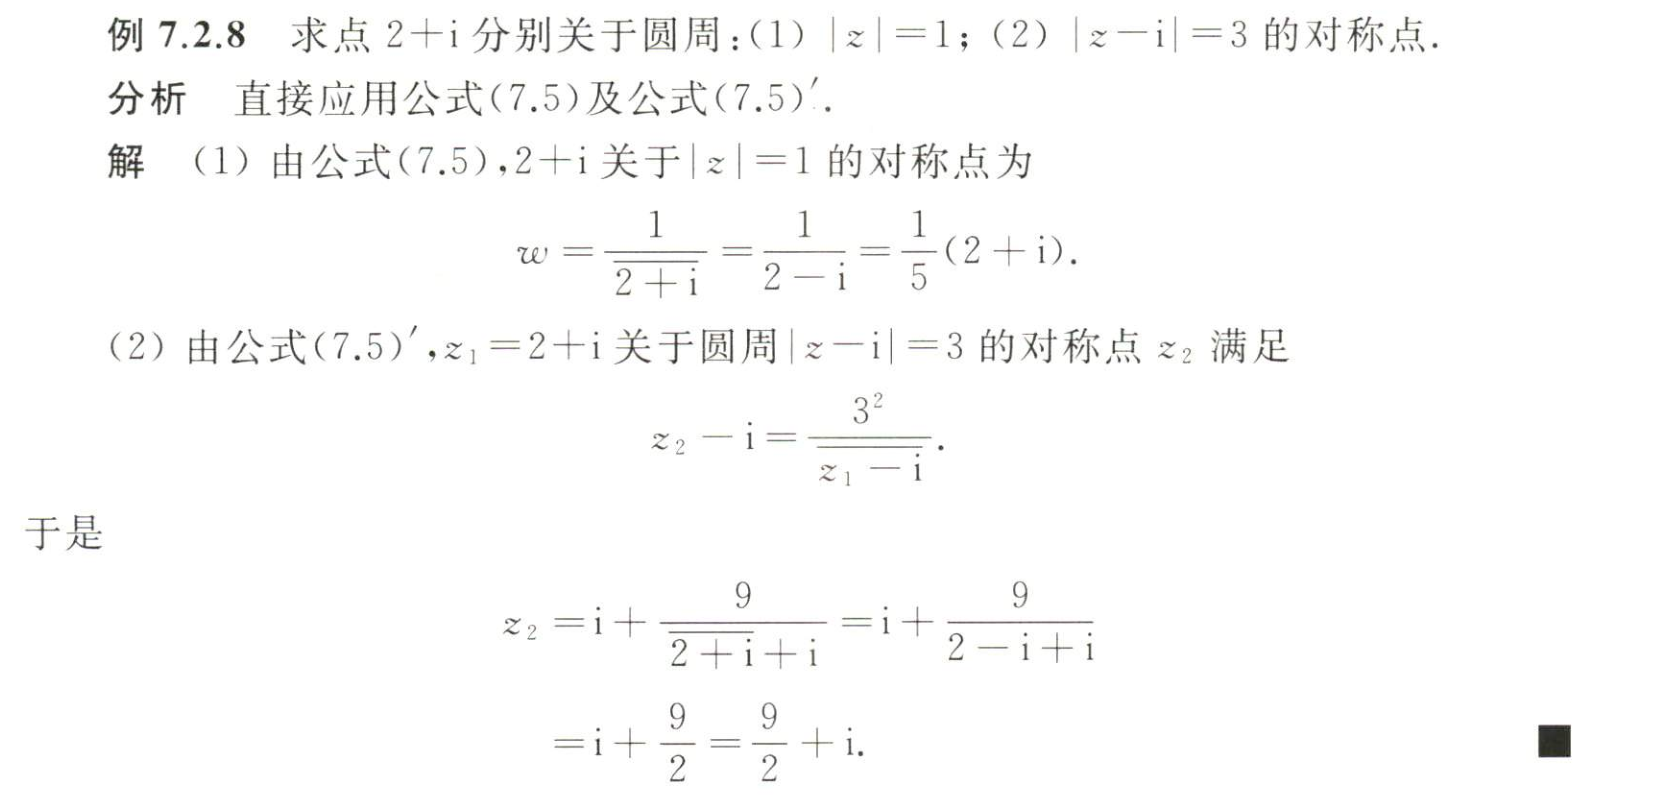
\includegraphics[width=\textwidth]{2-共形映射-刷题-2025060921.png}
% \caption{}
\label{}
\end{figure}

\begin{figure}[H]
\centering
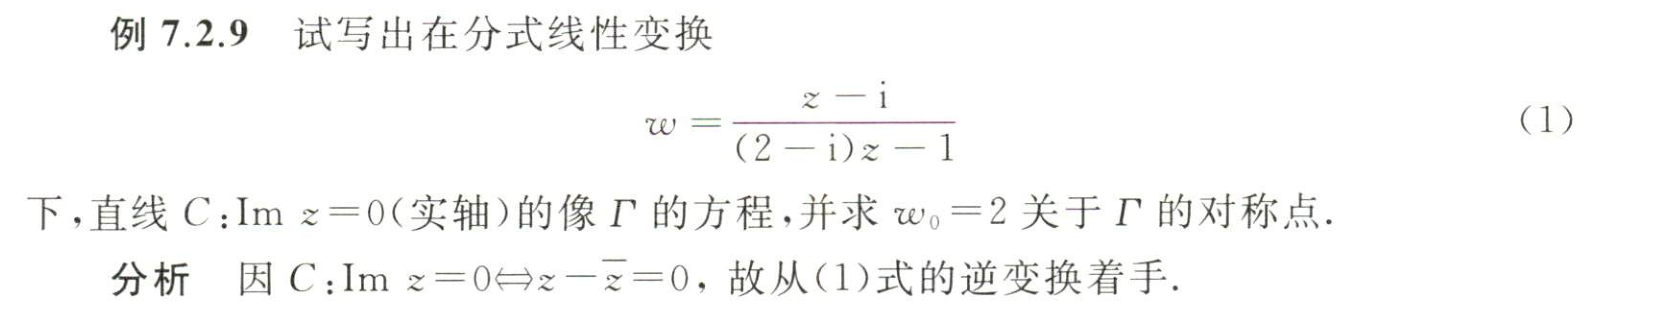
\includegraphics[width=\textwidth]{3-共形映射-刷题-2025060921.png}
% \caption{}
\label{}
\end{figure}
\begin{figure}[H]
\centering
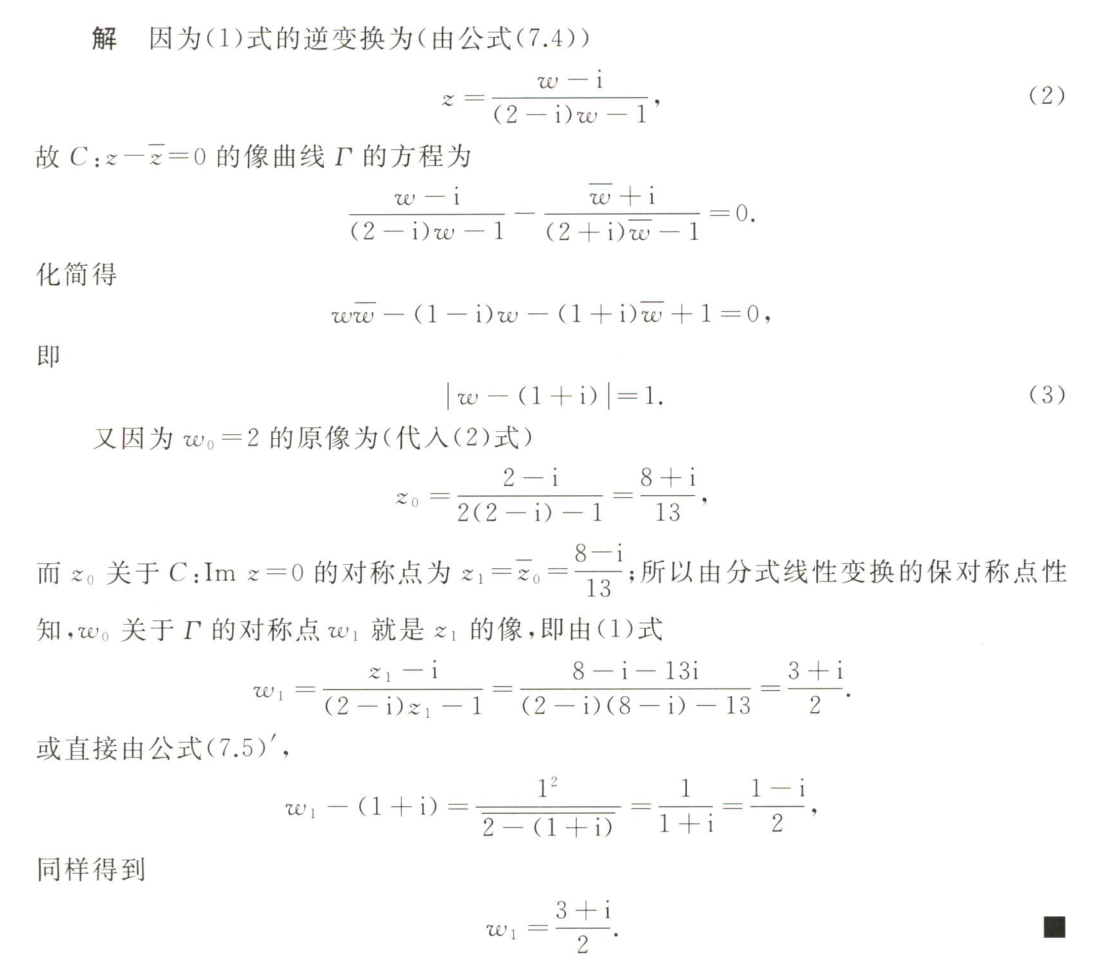
\includegraphics[width=\textwidth]{4-共形映射-刷题-2025060921.png}
% \caption{}
\label{}
\end{figure}

\subsection{特殊的分式线性映射}

\subsubsection{上半平面到上半平面}

\begin{figure}[H]
\centering
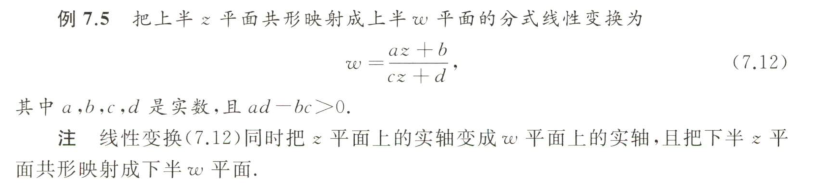
\includegraphics[width=\textwidth]{5-共形映射-刷题-2025060921.png}
% \caption{}
\label{}
\end{figure}

\subsubsection{上半平面到单位圆}

\begin{figure}[H]
\centering
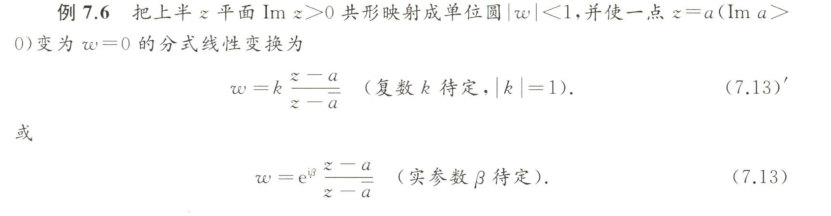
\includegraphics[width=\textwidth]{6-共形映射-刷题-2025060921.png}
% \caption{}
\label{}
\end{figure}

\subsubsection{单位圆到单位圆}

\begin{figure}[H]
\centering
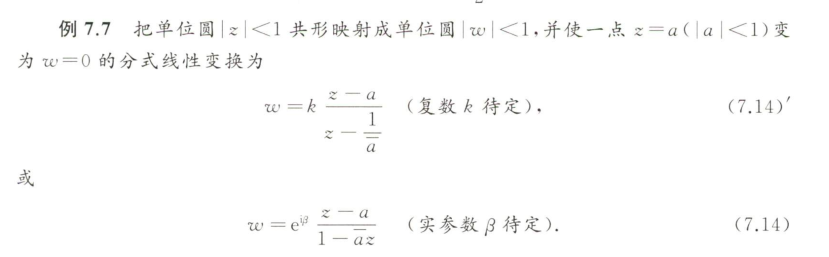
\includegraphics[width=\textwidth]{7-共形映射-刷题-2025060921.png}
% \caption{}
\label{}
\end{figure}

\subsection{固定两个点和图形的共形映射}

\begin{figure}[H]
\centering
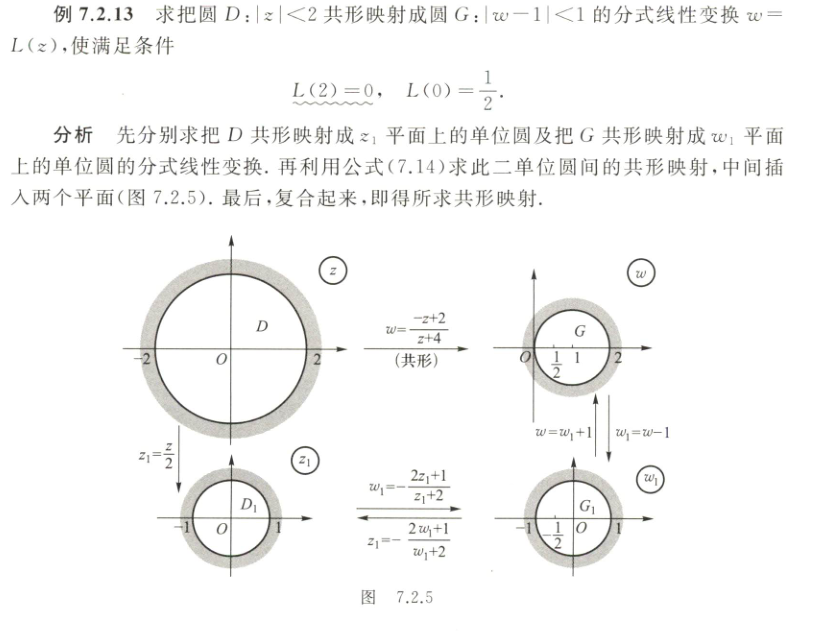
\includegraphics[width=\textwidth]{8-共形映射-刷题-2025060921.png}
% \caption{}
\label{}
\end{figure}

\begin{figure}[H]
\centering
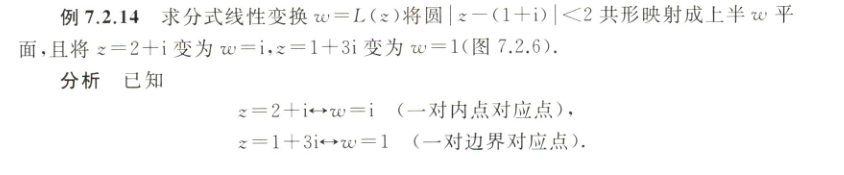
\includegraphics[width=\textwidth]{9-共形映射-刷题-2025060921.png}
% \caption{}
\label{}
\end{figure}
\begin{figure}[H]
\centering
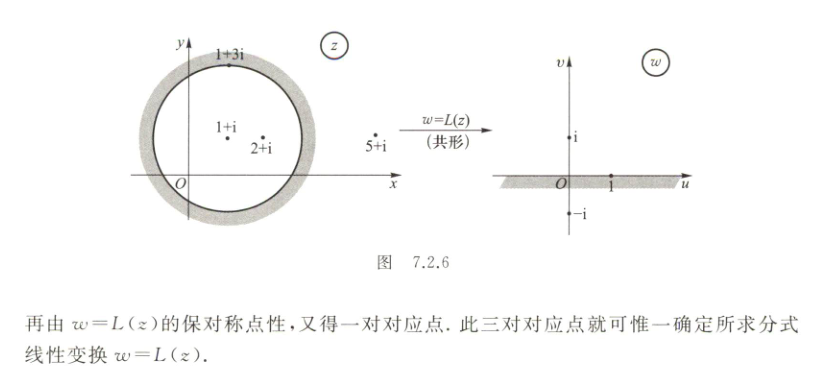
\includegraphics[width=\textwidth]{10-共形映射-刷题-2025060921.png}
% \caption{}
\label{}
\end{figure}

\subsection{初等函数的共形映射}

\subsubsection{幂函数:角形到角形}

\begin{figure}[H]
\centering
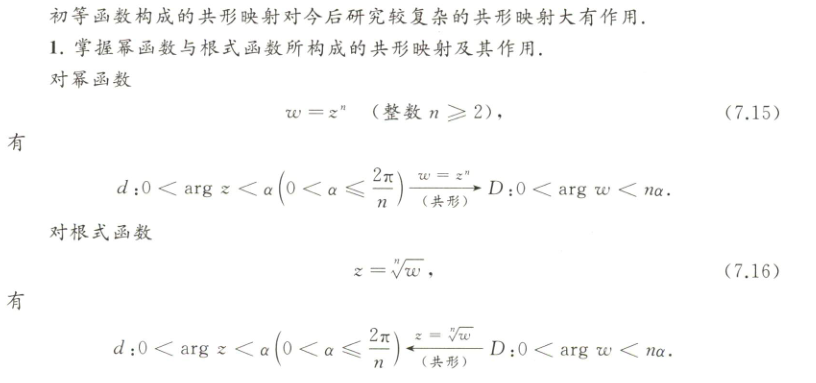
\includegraphics[width=\textwidth]{11-共形映射-刷题-2025060921.png}
% \caption{}
\label{}
\end{figure}

\subsubsection{指数函数:带形到角形}

\begin{figure}[H]
\centering
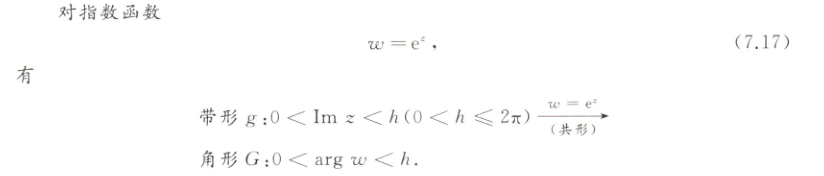
\includegraphics[width=\textwidth]{12-共形映射-刷题-2025060921.png}
% \caption{}
\label{}
\end{figure}

\subsubsection{对数函数:角形到带形}

\begin{figure}[H]
\centering
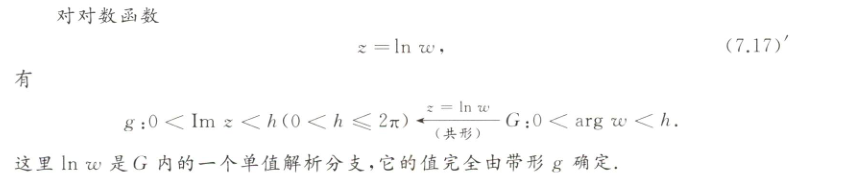
\includegraphics[width=\textwidth]{13-共形映射-刷题-2025060921.png}
% \caption{}
\label{}
\end{figure}

\subsection{带有割痕的共形映射}

\begin{figure}[H]
\centering
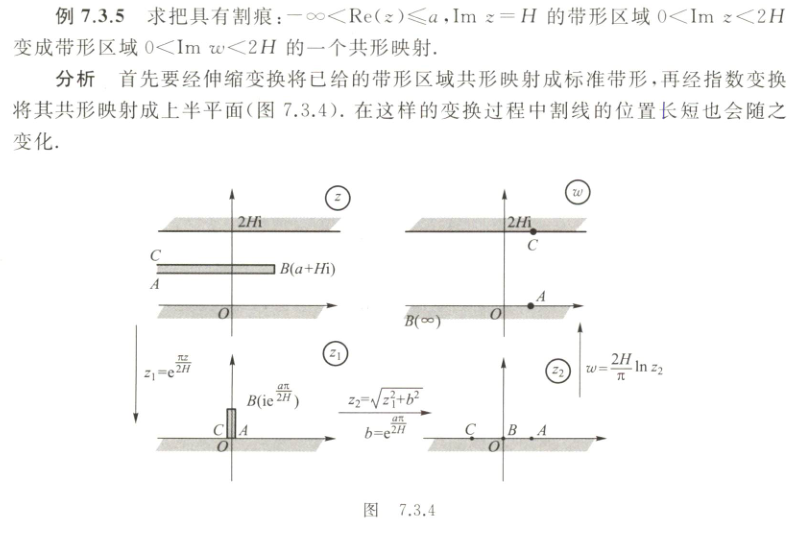
\includegraphics[width=\textwidth]{14-共形映射-刷题-2025060921.png}
% \caption{}
\label{}
\end{figure}

\subsection{两角形区域到角形}

\begin{figure}[H]
\centering
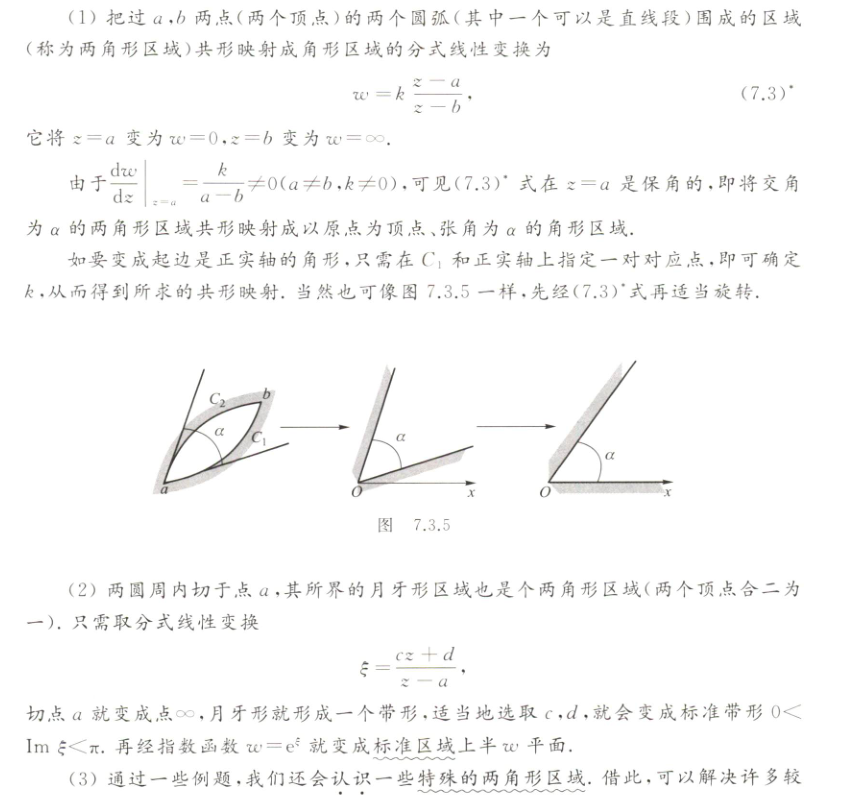
\includegraphics[width=\textwidth]{共形映射-刷题-2025060922.png}
% \caption{}
\label{}
\end{figure}

\subsubsection{可以利用两角形区域映射来理解}

\begin{figure}[H]
\centering
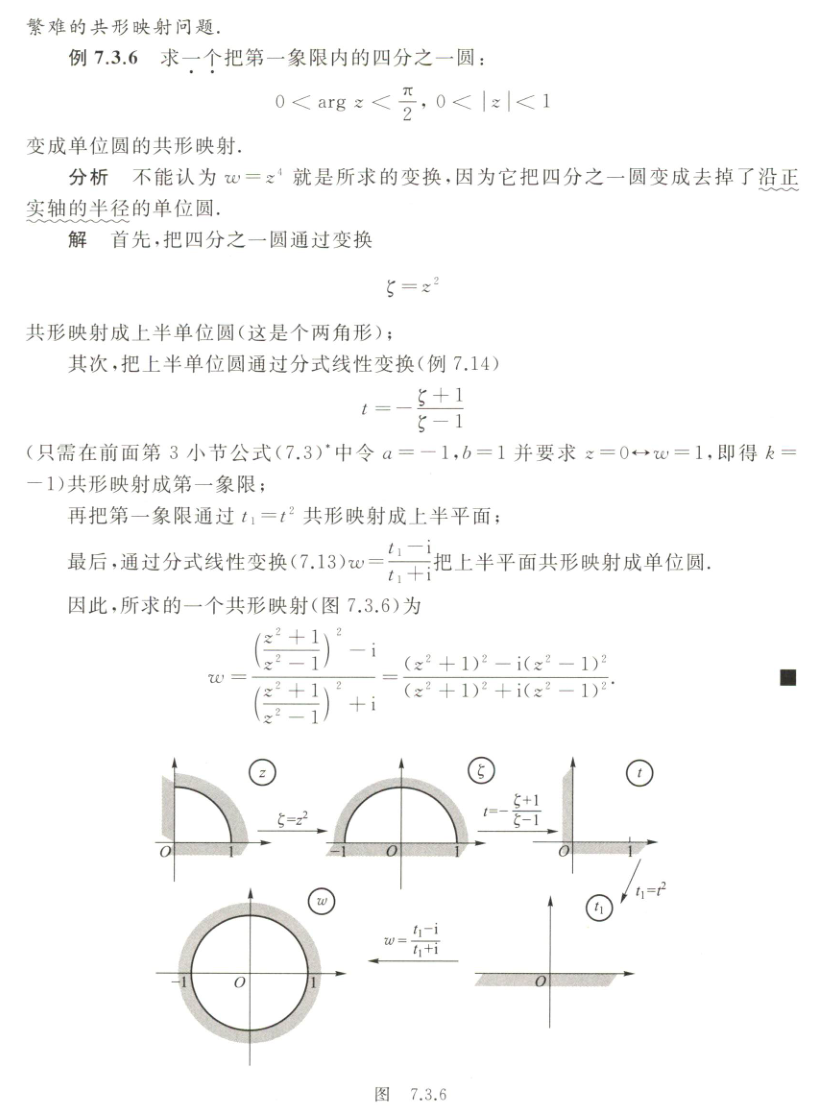
\includegraphics[width=\textwidth]{1-共形映射-刷题-2025060922.png}
% \caption{}
\label{}
\end{figure}

\begin{figure}[H]
\centering
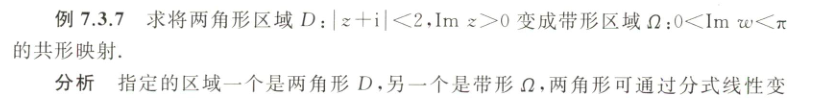
\includegraphics[width=\textwidth]{2-共形映射-刷题-2025060922.png}
% \caption{}
\label{}
\end{figure}
\begin{figure}[H]
\centering
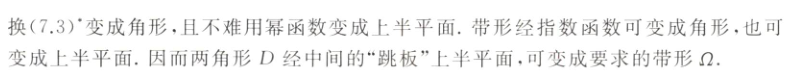
\includegraphics[width=\textwidth]{3-共形映射-刷题-2025060922.png}
% \caption{}
\label{}
\end{figure}
\begin{figure}[H]
\centering
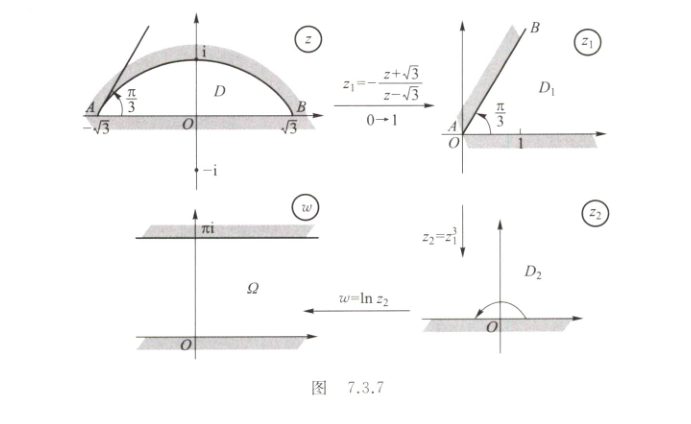
\includegraphics[width=\textwidth]{4-共形映射-刷题-2025060922.png}
% \caption{}
\label{}
\end{figure}

\subsection{月牙形的共形映射}

\begin{figure}[H]
\centering
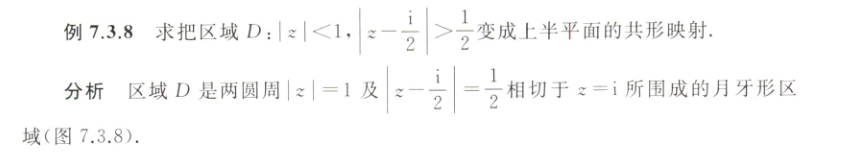
\includegraphics[width=\textwidth]{5-共形映射-刷题-2025060922.png}
% \caption{}
\label{}
\end{figure}
\begin{figure}[H]
\centering
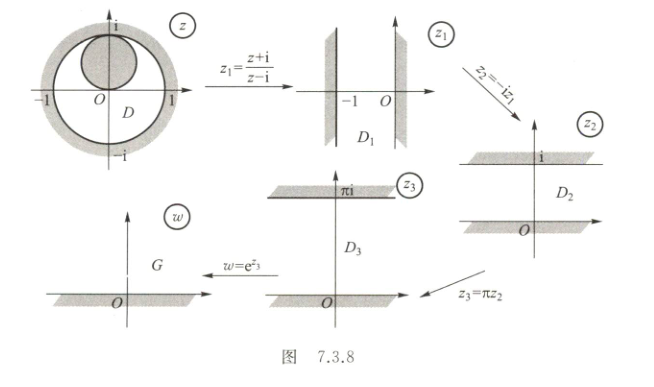
\includegraphics[width=\textwidth]{6-共形映射-刷题-2025060922.png}
% \caption{}
\label{}
\end{figure}
\begin{figure}[H]
\centering
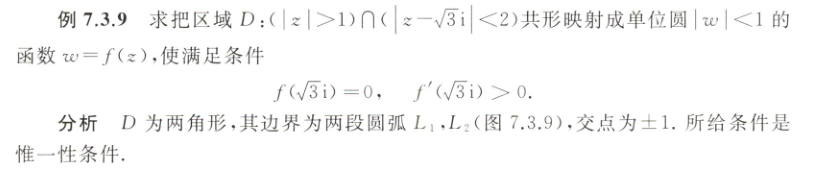
\includegraphics[width=\textwidth]{7-共形映射-刷题-2025060922.png}
% \caption{}
\label{}
\end{figure}
\begin{figure}[H]
\centering
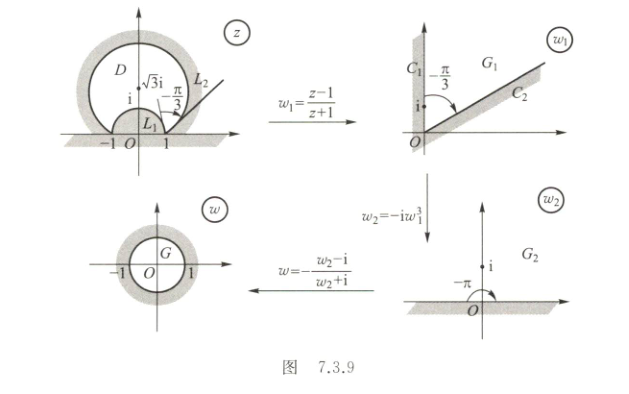
\includegraphics[width=\textwidth]{8-共形映射-刷题-2025060922.png}
% \caption{}
\label{}
\end{figure}

\subsection{茹科夫斯基变换}
\[
w=\frac{1}{2}\left( z+\frac{1}{z} \right)
\]
它把 $\lvert z \rvert=1$ 内部和外部都共形映射为扩充 $w$ 平面上去掉 $-1\leq \mathrm{Re}w\leq1,\text{Im }w=0$ 的区域,把上(下)半单位圆共形映射成下(上)半 $w$ 平面,把上(下)半单位圆周变成线段 $[-1,1]$ 的下(上)岸.

\begin{figure}[H]
\centering
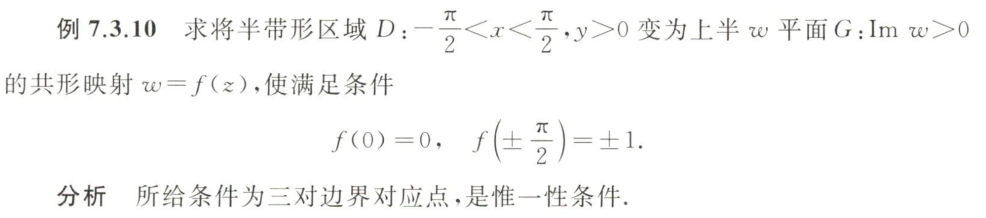
\includegraphics[width=\textwidth]{9-共形映射-刷题-2025060922.png}
% \caption{}
\label{}
\end{figure}
\begin{figure}[H]
\centering
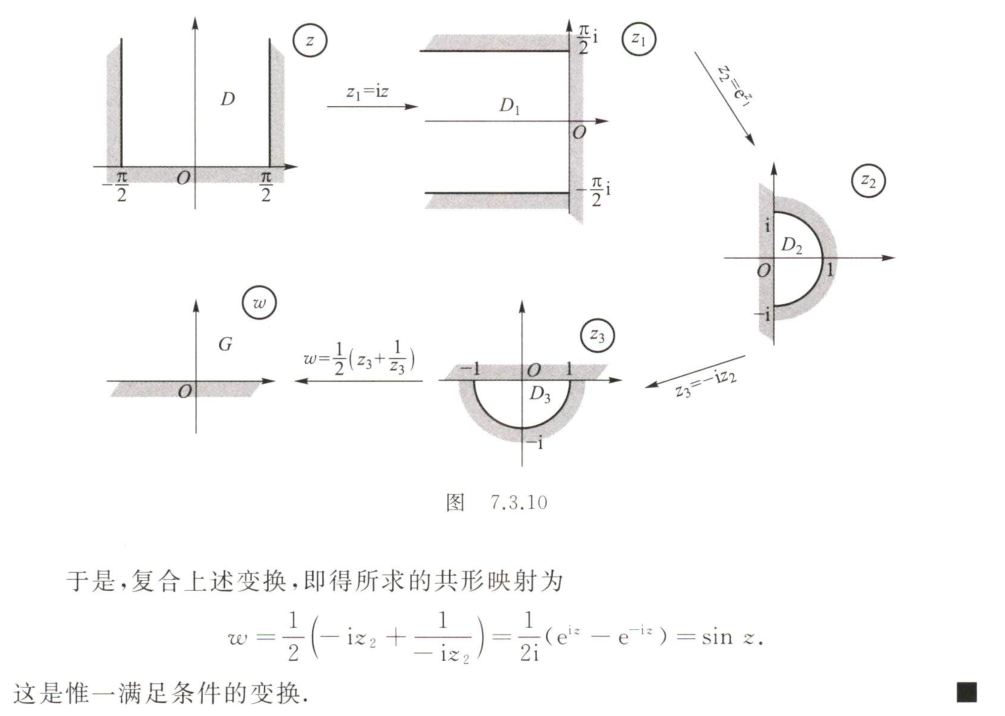
\includegraphics[width=\textwidth]{10-共形映射-刷题-2025060922.png}
% \caption{}
\label{}
\end{figure}

\begin{remark}
从上面的例题,我们易于想到,要求把一个区域 $D$ 变成区域 $G$ 的共形映射,如果能直接把函数求出最好;一般则是把 $D$ 或 $G$ ,或把 $D$ 与 $G$ 都设法变成上半平面或单位圆,然后求出共形映射.这里上半平面或单位圆起着中间或桥梁的作用,也称为标准区域。
\end{remark}
\subsubsection{逆变换 \texorpdfstring{$\sqrt{ \zeta^{2}-1 }+\zeta$}{sqrt zeta^2-1 +zeta}}

$\left.\sqrt{ \zeta^{2}-1 }\right|_{\zeta=i}=\sqrt{ 2 }i$ 那一支将 $\mathbb{C}\setminus[-1,1]$ 映射到 $\lvert w \rvert>1$. $\left.\sqrt{ \zeta^{2}-1 }\right|_{\zeta=i}=-\sqrt{ 2 }i$ 那一支将 $\mathbb{C}\setminus[-1,1]$ 映射到 $\lvert w \rvert<1$.

\section{复杂的图形之间的映射}

See Problems and Solutions in Mathematics (Jixiu Chen, et al.)

\subsection{单位圆盘到去掉 \texorpdfstring{$[0,1)$}{[0,1)} 的圆盘}

\begin{exercise}
Find a one-to-one holomorphic map from the unit disk $\{|z|<1\}$ ont slit disk $\{|w|<1\}-\{[0,1)\}$.
\end{exercise}
We construct the map by the following steps:
\[
z_1=  \phi_1(z)=i \frac{z+1}{z-1}:\{z:|z|<1\} \rightarrow\left\{z_1: \operatorname{Im} z_1<0\right\}
\]
\[
\begin{aligned}
z_2=  \phi_2\left(z_1\right)=\sqrt{z_1^2-1}+z_1 \quad\left(\left.\sqrt{z_1^2-1}\right|_{z_1=-i}=\sqrt{2} i\right):\\
\left\{z_1: \operatorname{Im} z_1<0\right\} \rightarrow\left\{z_2:\left|z_2\right|<1 \text { and } \operatorname{Im} z_2>0\right\}
\end{aligned}
\]
\[
w=  \phi_3\left(z_2\right)=z_2^2:\left\{z_2:\left|z_2\right|<1 \text { and } \operatorname{Im} z_2>0\right\} \rightarrow
\{w:|w|<1\} \backslash\{w: \operatorname{Im} w=0,0 \leq \operatorname{Re} w<1\} .
\]
Then $w=\phi_3 \circ \phi_2 \circ \phi_1(z)=f(z)$ is a one-to-one holomorphic map from the unit disk $\{|z|<1\}$ onto the slit disk $\{|w|<1\} \backslash\{[0,1)\}$.

\subsection{两区域之间的共形映射}

\begin{exercise}[Illinois]
\begin{enumerate}
		\item Find a function $f$ that conformally maps the region $\{z:|\arg z|<1\}$ one-to-one onto the region $\{w:|w|<1\}$. Show that the function you have found satisfies the required conditions.
		\item Is it possible to require that $f(1)=0$ and $f(2)=\frac{1}{2}$? If yes, give an explicit map; if No, explain why not.
	\end{enumerate}
\end{exercise}
\begin{proof}
(a) $\zeta=f_1(z)=z^{\frac{\pi}{2}}=e^{\frac{\pi}{2} \log z}(\log 1=0)$ is a conformal map of $\{z : |\arg z|<1\}$ onto $\{\zeta: \operatorname{Re} \zeta>0\}$, and $w=f_2(\zeta)=\frac{\zeta-1}{\zeta+1}$ is a conformal map of $\{\zeta: \operatorname{Re} \zeta>0\}$ onto $\{w:|w|<1\}$.

Hence
\[
w=f(z)=f_2 \circ f_1(z)=\frac{z^{\frac{\pi}{2}}-1}{z^{\frac{\pi}{2}}+1}
\]
is a conformal map of $\{z:|\arg z|<1\}$ onto $\{w:|w|<1\}$ with $f(1)=0$ and $f(2)=\frac{2^{\frac{\pi}{2}}-1}{2^{\frac{\pi}{2}}+1}$.

(b) Suppose $\widetilde{w}=\widetilde{f}(z)$ is an arbitrary conformal map of $\{z:|\arg z|<1\}$ onto $\{\widetilde{w}:|\widetilde{w}|<1\}$ with $\widetilde{f}(1)=0$.

Then $w=F(\widetilde{w})=f \circ \widetilde{f}^{-1}(\widetilde{w})$ is a conformal map of $\{\widetilde{w}:|\widetilde{w}|<1\}$ onto $\{w:|w|<1\}$ with $F(0)=0$, and $\widetilde{w}=\widetilde{F}(w)=\widetilde{f} \circ f^{-1}(w)$ is a conformal map of $\{w:|w|<1\}$ onto $\{\widetilde{w}:|\widetilde{w}|<1\}$ with $\widetilde{F}(0)=0$.

By Schwarz's lemma, we have both $|F(\widetilde{w})| \leq|\widetilde{w}|$ and $|\widetilde{F}(w)| \leq|w|$, which implies that $|f(z)|=|\widetilde{f}(z)|$ for every $z \in\{z:|\arg z|<1\}$.

Since
\[
f(2)=\frac{2^{\frac{\pi}{2}}-1}{2^{\frac{\pi}{2}}+1}
\]
we cannot require that $\widetilde{f}(2)=\frac{1}{2}$.
\end{proof}

\subsection{共形映射类}

\begin{exercise}[Toronto]
\begin{enumerate}
		\item Find one 1-1 onto conformal map $f$ that sends the open quadrant $\{(x, y): x>0$ and $y>0\}$ onto the open lower half disc $\left\{(x, y): x^2+y^2<\right.$ 1 and $y<0\}$.
		\item Find all such $f$.
	\end{enumerate}
\end{exercise}
\begin{proof}

\begin{enumerate}
	\item Let $\zeta=\phi_1(z)=z^2$. It is a conformal map of $\{z=x+i y: x>$ 0 and $y>0\}$ onto $\{\zeta=\xi+i \eta: \eta>0\}$.
Let $w=\phi_2(\zeta)=\sqrt{\zeta^2-1}+\zeta$, where $\left.\sqrt{\zeta^2-1}\right|_{\zeta=i}=-\sqrt{2} i$. It is a conformal map of $\{\zeta=\xi+i \eta: \eta>0\}$ onto $\left\{w=u+i v: u^2+v^2<1\right.$ and $\left.v<0\right\}$.
Then $w=\phi_2 \circ \phi_1(z)=\sqrt{z^4-1}+z^2$, where $\left.\sqrt{z^4-1}\right|_{z=e^{\frac{\pi}{4} i}}=-\sqrt{2} i$ is a required conformal map.
	\item If $f$ is an arbitrary conformal map satisfying the condition of (1), then $\phi_2^{-1} \circ f \circ \phi_1^{-1}(\zeta)$ is a conformal map of the upper half plane onto itself, which can be represented by $\psi(\zeta)=\frac{a \zeta+b}{c \zeta+d}$, where $a, b, c, d \in \mathbb{R}, a d-b c>0$. Hence $f$ can be written as $\phi_2 \circ \psi \circ \phi_1(z)$.
\end{enumerate}

\end{proof}

\subsection{不等式估计 \texorpdfstring{$\lvert f'(0) \rvert$}{|f'(0)|} (利用 Schwarz 引理)}

\begin{exercise}
\begin{figure}[H]
\centering
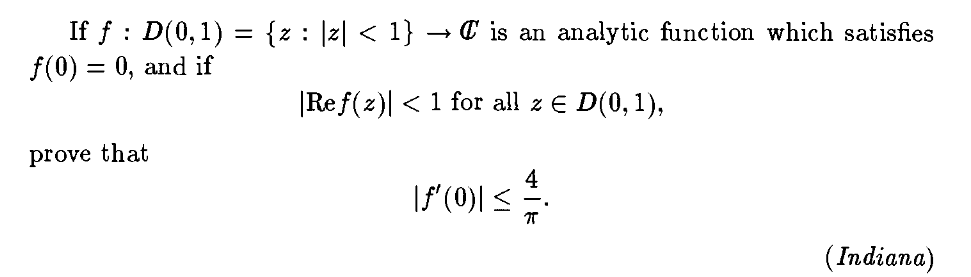
\includegraphics[width=\textwidth]{共形映射-刷题-2025061021.png}
% \caption{}
\label{}
\end{figure}
\end{exercise}
\begin{figure}[H]
\centering
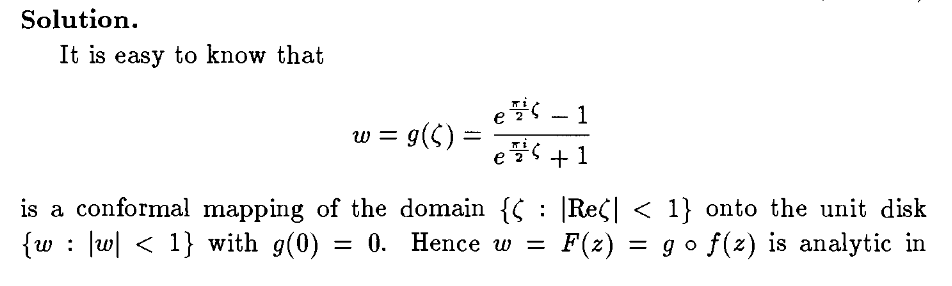
\includegraphics[width=\textwidth]{1-共形映射-刷题-2025061021.png}
% \caption{}
\label{}
\end{figure}
\begin{figure}[H]
\centering
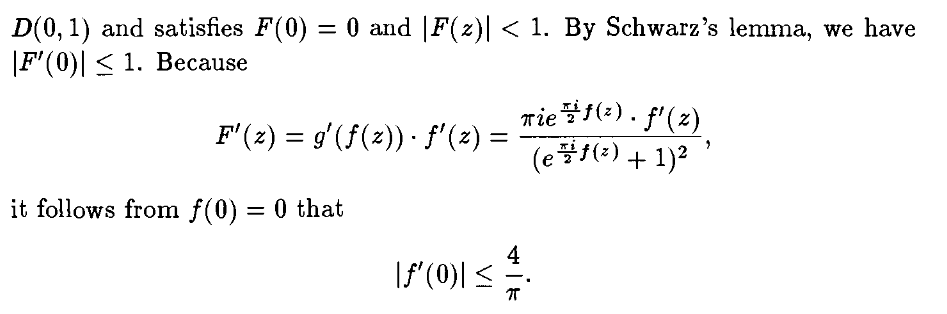
\includegraphics[width=\textwidth]{2-共形映射-刷题-2025061021.png}
% \caption{}
\label{}
\end{figure}

\subsection{给定约束条件下的函数极值估计}

\begin{exercise}
\begin{figure}[H]
\centering
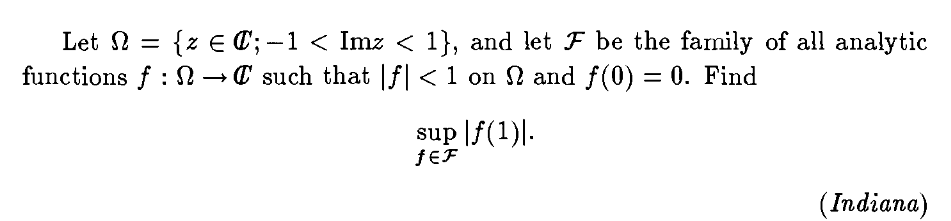
\includegraphics[width=\textwidth]{3-共形映射-刷题-2025061021.png}
% \caption{}
\label{}
\end{figure}
\end{exercise}
\begin{figure}[H]
\centering
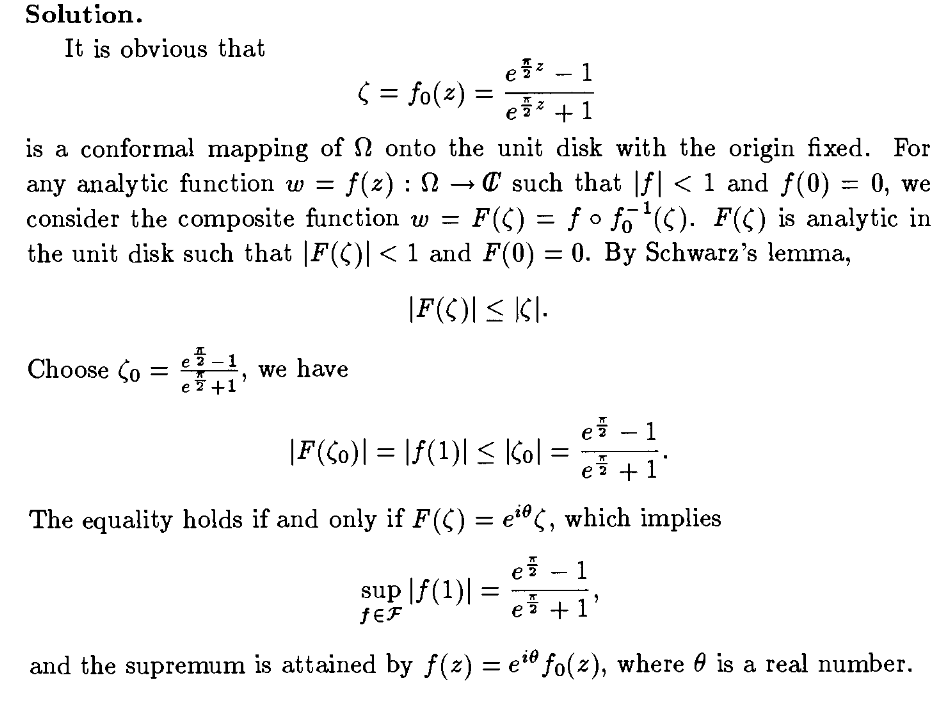
\includegraphics[width=\textwidth]{4-共形映射-刷题-2025061021.png}
% \caption{}
\label{}
\end{figure}

\begin{exercise}
\begin{figure}[H]
\centering
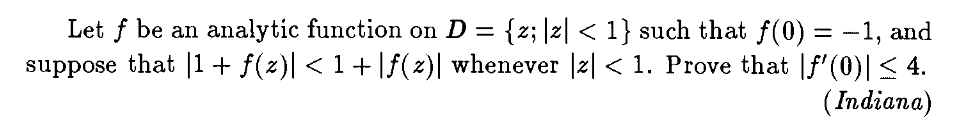
\includegraphics[width=\textwidth]{5-共形映射-刷题-2025061021.png}
% \caption{}
\label{}
\end{figure}
\end{exercise}
\begin{figure}[H]
\centering
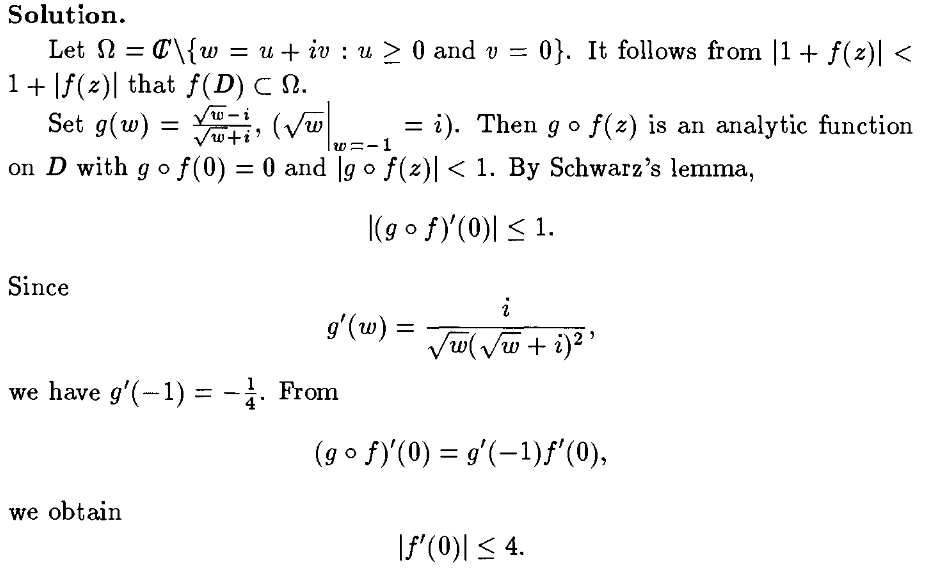
\includegraphics[width=\textwidth]{6-共形映射-刷题-2025061021.png}
% \caption{}
\label{}
\end{figure}

\begin{exercise}
\begin{figure}[H]
\centering
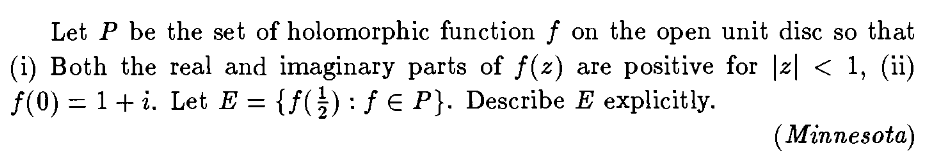
\includegraphics[width=\textwidth]{共形映射-刷题-2025061023.png}
% \caption{}
\label{}
\end{figure}
\end{exercise}
\begin{figure}[H]
\centering
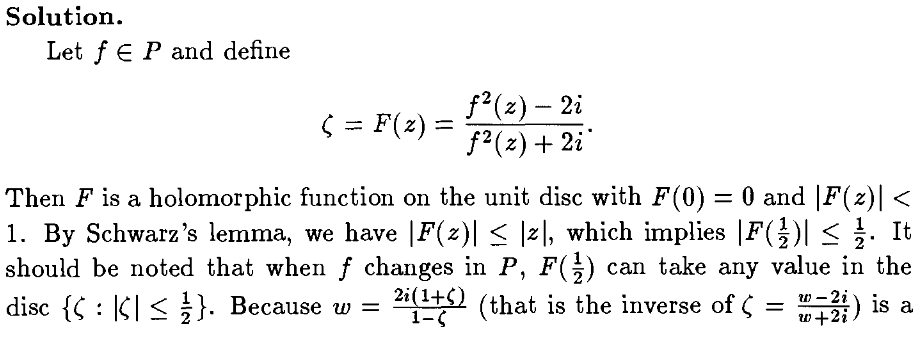
\includegraphics[width=\textwidth]{1-共形映射-刷题-2025061023.png}
% \caption{}
\label{}
\end{figure}
\begin{figure}[H]
\centering
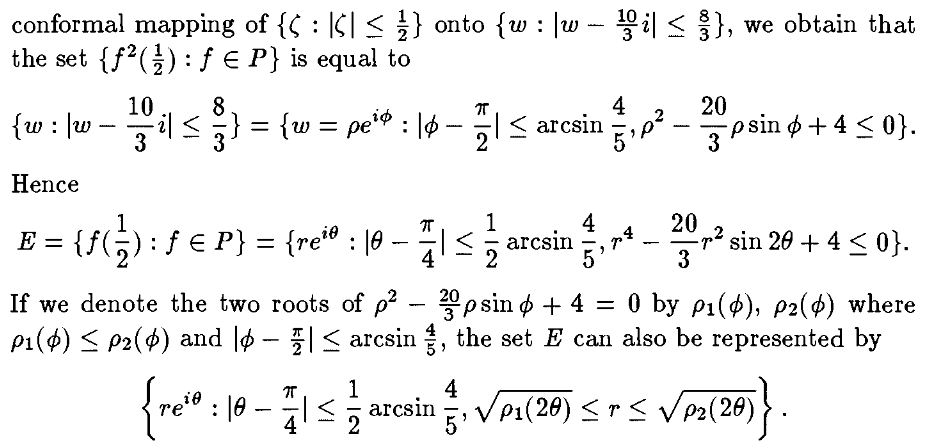
\includegraphics[width=\textwidth]{2-共形映射-刷题-2025061023.png}
% \caption{}
\label{}
\end{figure}

\subsection{幂等共形映射存在唯一不动点}

\begin{exercise}
\begin{figure}[H]
\centering
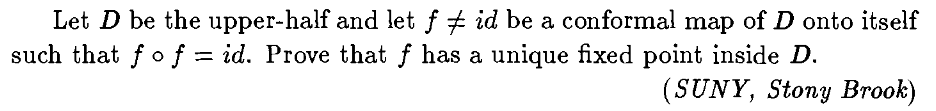
\includegraphics[width=\textwidth]{3-共形映射-刷题-2025061023.png}
% \caption{}
\label{}
\end{figure}
\end{exercise}
\begin{figure}[H]
\centering
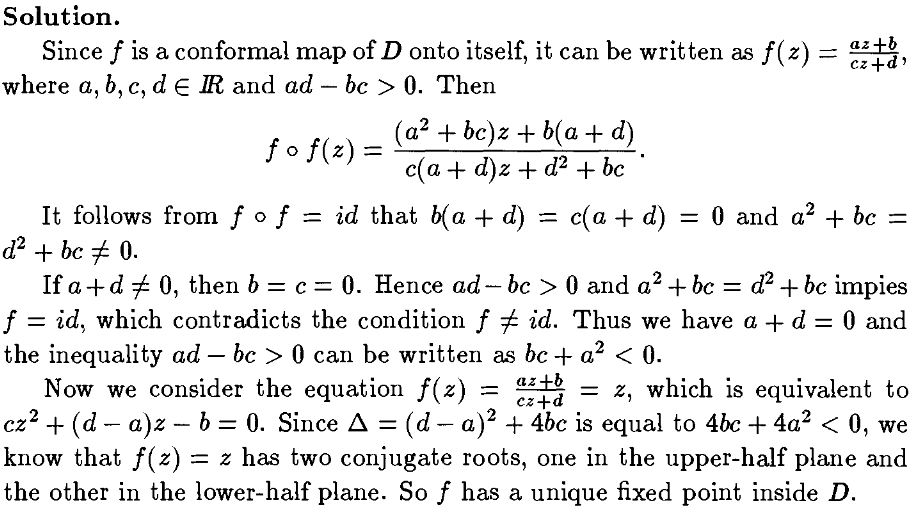
\includegraphics[width=\textwidth]{4-共形映射-刷题-2025061023.png}
% \caption{}
\label{}
\end{figure}

\subsection{证明满足 \texorpdfstring{$\text{Re }f'(z)>0$}{textRe f'(z)>0} 的 \texorpdfstring{$f$}{f} 为单射}

\begin{exercise}
\begin{figure}[H]
\centering
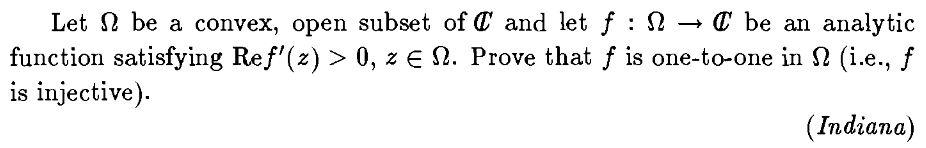
\includegraphics[width=\textwidth]{5-共形映射-刷题-2025061023.png}
% \caption{}
\label{}
\end{figure}
\end{exercise}
\begin{figure}[H]
\centering
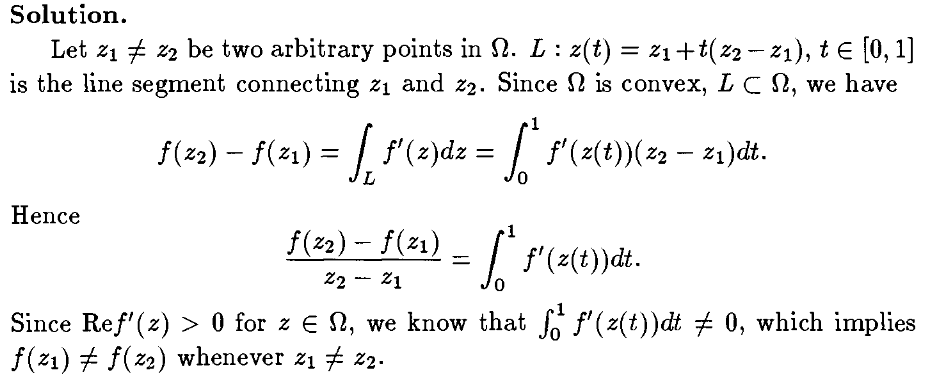
\includegraphics[width=\textwidth]{6-共形映射-刷题-2025061023.png}
% \caption{}
\label{}
\end{figure}

\subsection{考虑多项式的根}

\begin{exercise}
\begin{figure}[H]
\centering
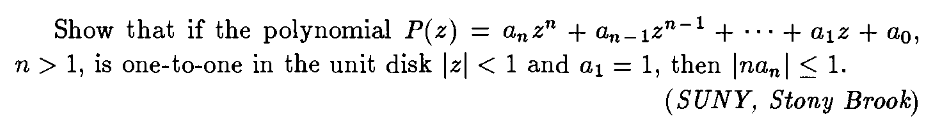
\includegraphics[width=\textwidth]{8-共形映射-刷题-2025061023.png}
% \caption{}
\label{}
\end{figure}
\end{exercise}
\begin{figure}[H]
\centering
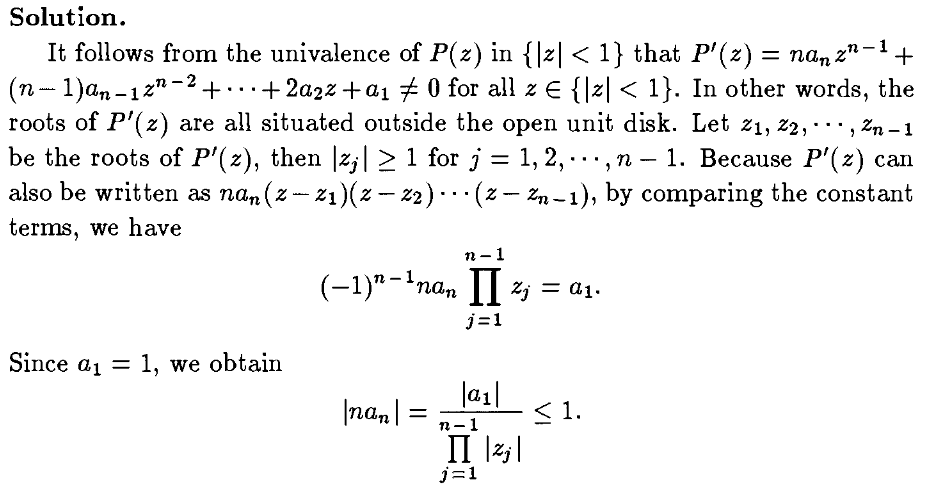
\includegraphics[width=\textwidth]{9-共形映射-刷题-2025061023.png}
% \caption{}
\label{}
\end{figure}
